%! tex root = ../master.tex

\newcommand{\excreturn}{EXC\_RETURN}

\chapter{System Implementation}
\todo[inline, color=green]
{INTRO, to be reviewed}
This chapter deals with how the system\textquotesingle s functionalities 
are implemented. Diagrams will be included when necessary, as well as code 
snippets for the interesting parts of the program. In the end, all these
will be reviewed and compared with the actual requirements of the standard.


\section{Hardware}

As mentioned in the previous chapter, the hardware used for this project 
is a MINI-M4 board from MikroElectronica. This is build around an
STM32F415RG microcontroller produced by STMicroelectronics. Besides
this, the board contains two crystal oscillators, two LEDs, a reset 
button and the peripherals for supplying power via a microUSB connector.
Some of the GPIOs are break through using external pins.
These pins were soldered to the board, and this was setup on a breadboard
for practicality, as seen in \ref{fig:photo1}.

\begin{figure}[H]
\begin{subfigure}{0.5\textwidth}
  \centering
  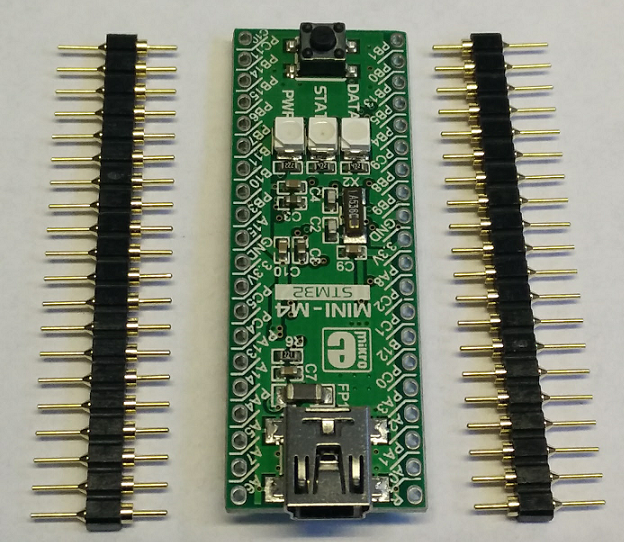
\includegraphics[width=3cm]{hardware/board_not_soldered.png}
  \caption{MINI-M4 before soldernig}
  \label{fig:sub1}
\end{subfigure}%
\begin{subfigure}{0.5\textwidth}
  \centering
  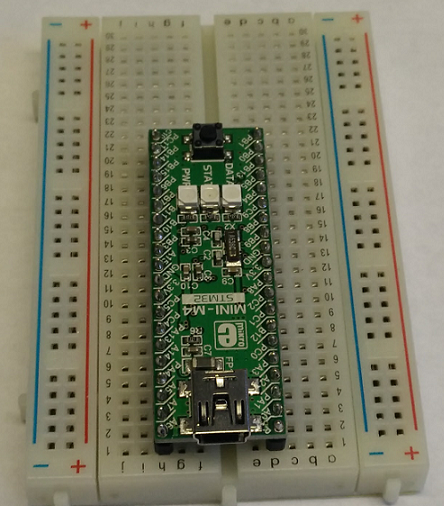
\includegraphics[width=3cm]{hardware/board_on_breadboard.png}
  \caption{MINI-M4 on a breadboard}
  \label{fig:sub2}
\end{subfigure}
\caption{Preparation of the board}
\label{fig:photo1}
\end{figure}

For programming and debugging the board the JTAG interface was used.
This had to be connected to certain pins of the board. In order to get 
feedback from the board, a serial connection was used, which requires two
more lines to it. This can be seen in the next figure.

\begin{figure}[H]
\centering
\begin{subfigure}{.5\textwidth}
  \centering
  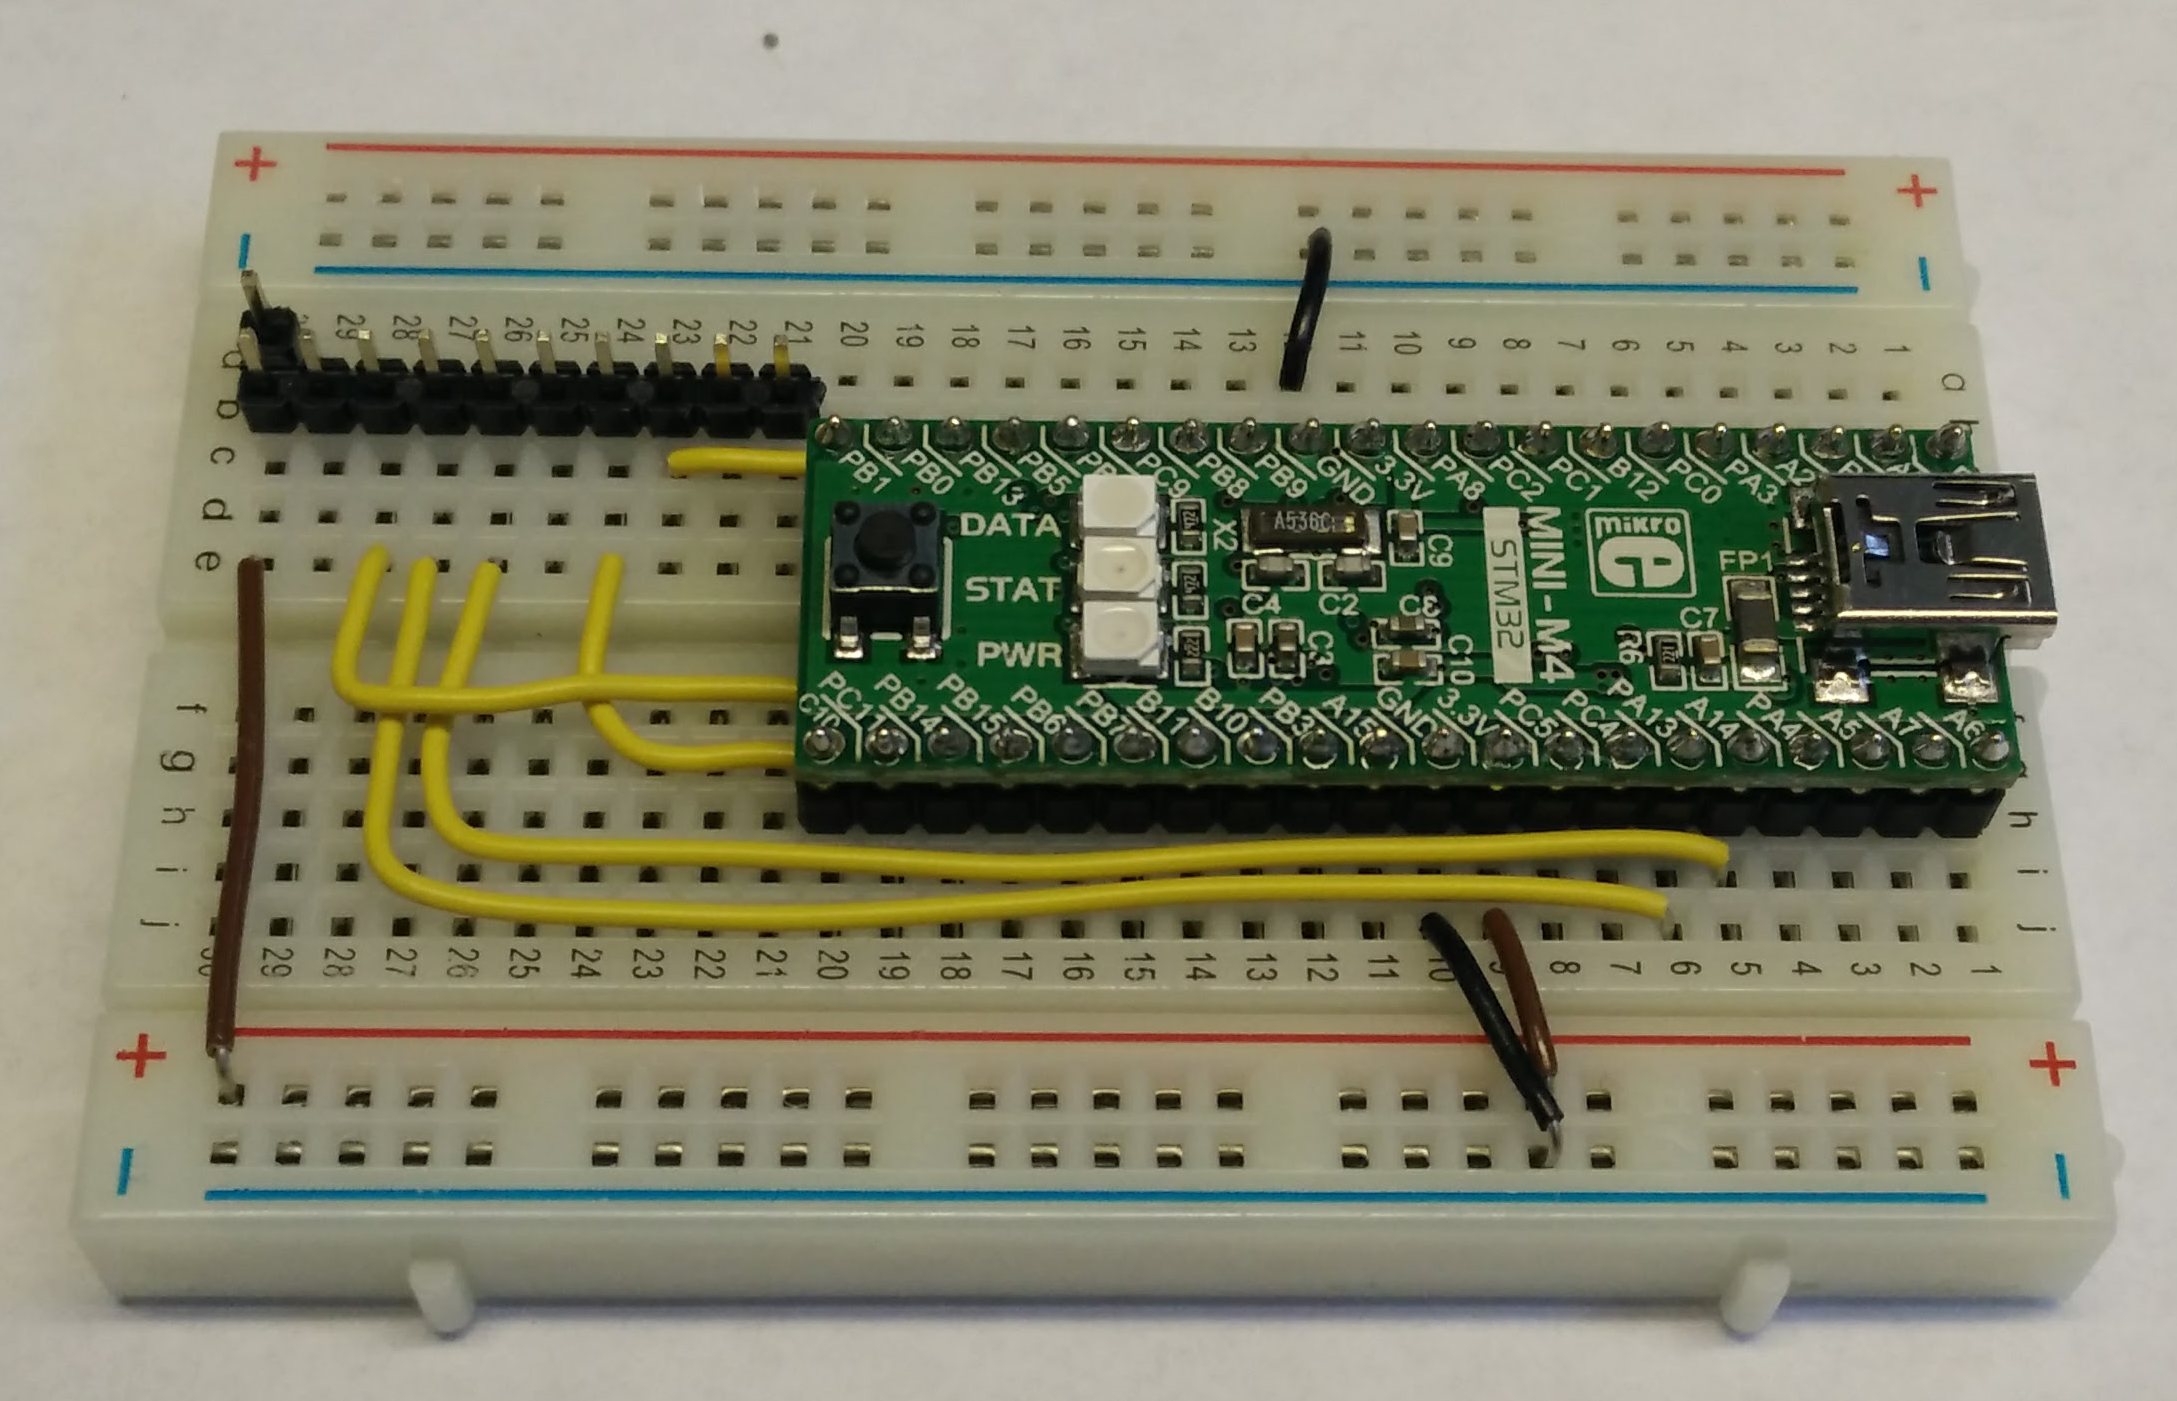
\includegraphics[width=.4\linewidth]{hardware/board_with_jtag_lines}
  \caption{The JTAG lines}
  \label{fig:sub1}
\end{subfigure}%
\begin{subfigure}{.5\textwidth}
  \centering
  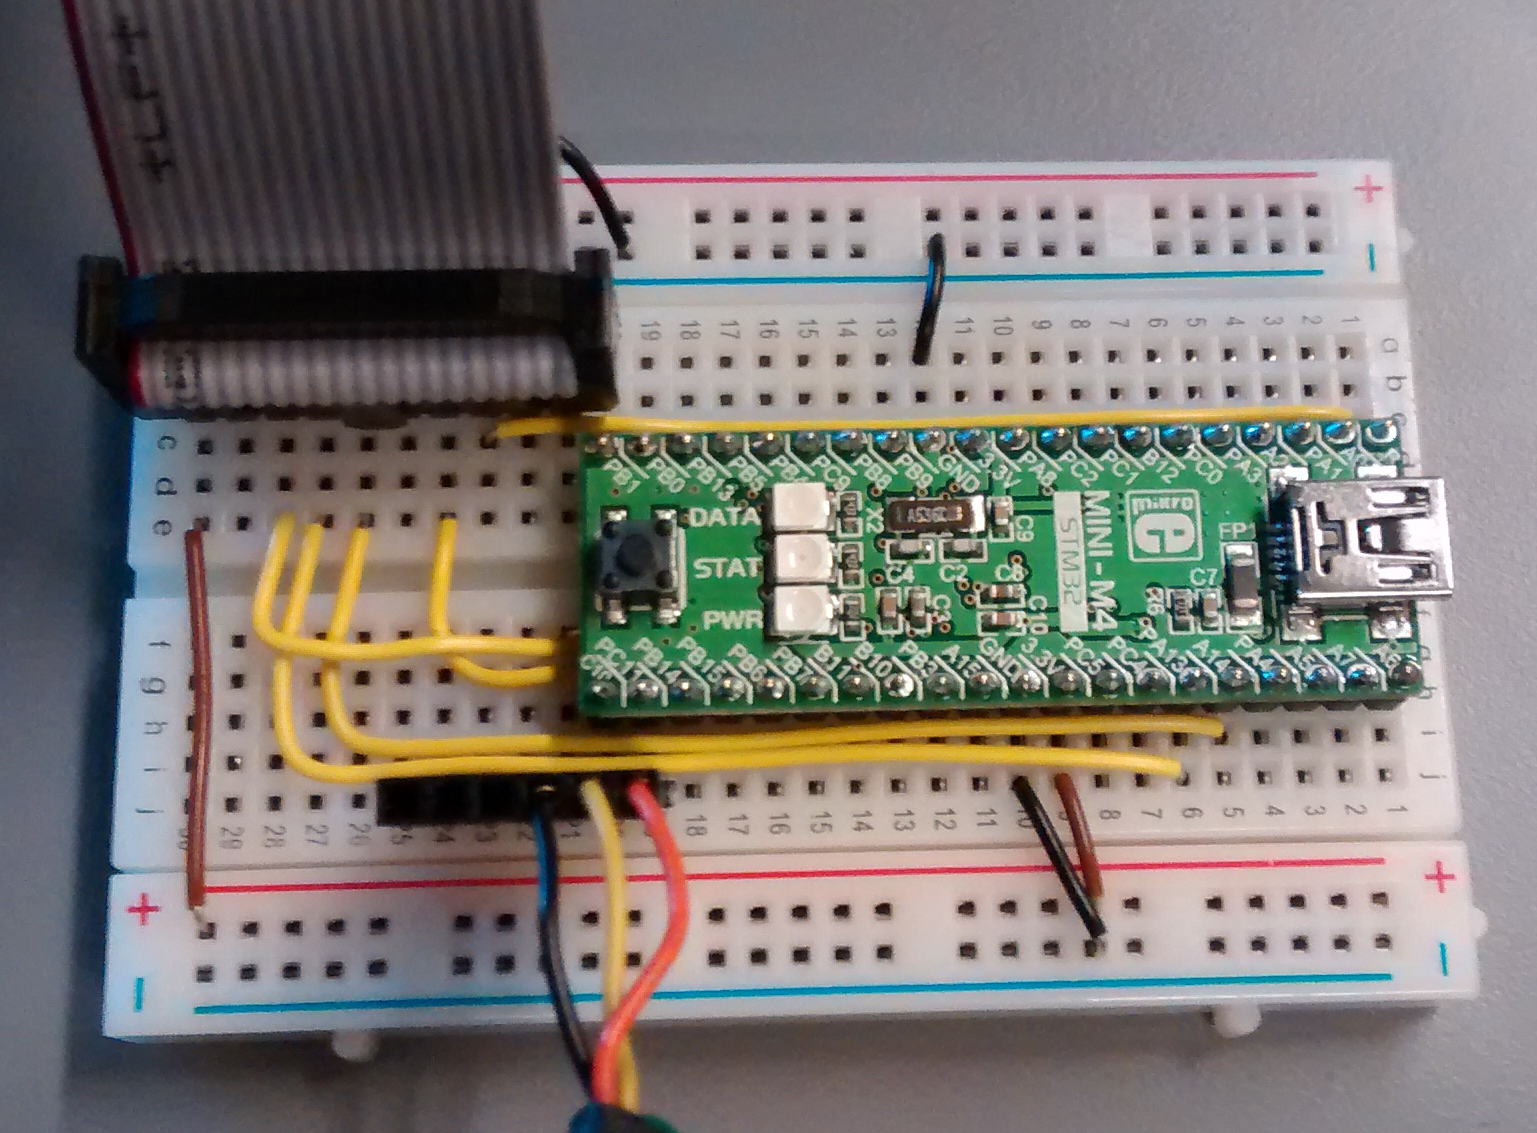
\includegraphics[width=.4\linewidth]{hardware/board_with_jtag_and_serial}
  \caption{Both the JTAG and serial interfaces}
  \label{fig:sub2}
\end{subfigure}
\caption{Connecting the board}
\label{fig:photo2}
\end{figure}

After this, the board was ready to be used in the development process.
The only drawback of this setup, is that it requires three USB ports:
power for the board, the JTAG interface, and the serial communication.

\subsection{JTAG Interface}
\label{ssec:JTAG_Interface}


\section{Toolchain}
To write, compile and load code to the embedded platform, a regular computer is used with an editor of ones own choice, a compiler running on Linux and a programmer unit to transmit the code by the JTAG interface (\ref{ssec:JTAG_Interface}).
Even though Linux is used in the process, compiling and loading the code from Windows is also supported. OSX should also work with only small ajustments, being a UNIX system compatible with many Linux tools.
In the rest of the section the toolchain and source structure is explained.

\subsection{CMAKE}
CMake when compiling is used as an intermediate layer when

\subsection{GCC}

\subsubsection{Compiler Flags}

\subsubsection{Linker Script}

\subsection{OpenOCD}

\subsection{GDB}

\subsection{Compiling the Code}


\section{Source Structure}


\section{Drivers}

\subsection{System clock}
\begin{figure}[H]
\centering
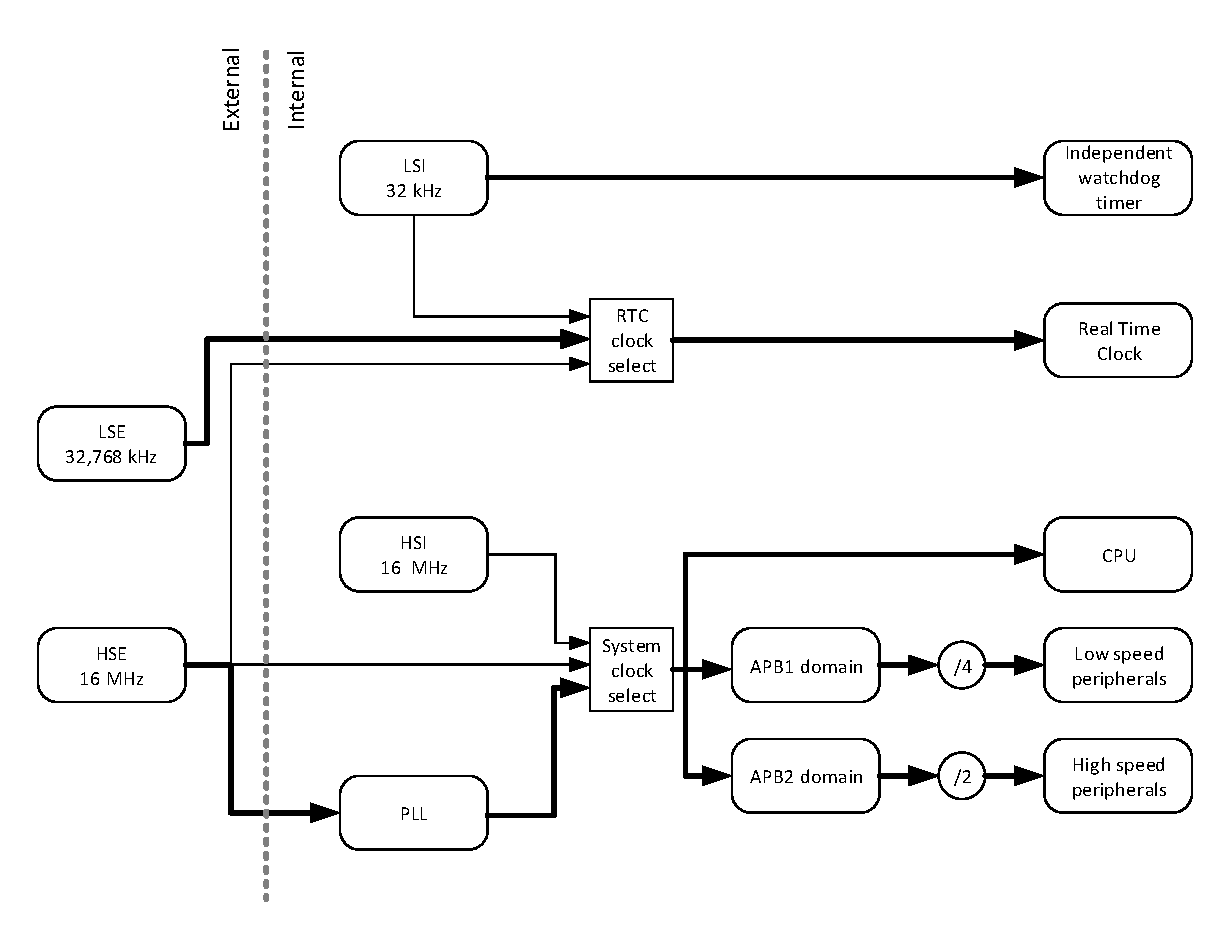
\includegraphics[width=\textwidth]{system_clock.pdf}
\captionof{figure}{An advanced system overview}
\label{fig:advanced_system}
\end{figure}


\subsection{Other peripherals}

\section{Drivers}


\subsection{UART}
The UART sets the speed of the transmission and reception of the information between the STM32 and the outside. The communication is made by one character at a time. The transmission is activated by the interrupts and it can happen both ways simultaneously, or one way at a time. An UART has a clock generator, that we set for 16Mz, input and output registers, transmit/receive control, read/write control logic, and transmit/receiver buffers.
It is also possible to communicate with the UART using a screen, getting some important output for debugging.

\subsection{Watchdog timer}
% \ http://electronics.stackexchange.com/questions/123080/independent-watchdog-iwdg-or-window-watchdog-wwdg
The STM32 MCU has two watchdog timers ready to reset the program, in case of an error.
The first one, is the independent watchdog timer, based on an independent oscillator (32 kHz).
When initialised, the watchdog timer receives a value, from which it starts counting down, using
the ticks from the crystal. In the meanwhile, the program has to reset this count, by refreshing 
the timer to the same value it used before. If this fails to happen, when the count reaches zero, 
the watchdog timer will react by restarting the board.
\\
The second watchdog timer, is called a window watchdog. In contrast to the independent watchdog, 
one can provide a time interval in which the timer has to be reset. Resetting the timer outside this interval(as well as not resetting it in the mentioned time window) would restart the program. It uses 
the system clock, which means that if this fails, the watchdog won't be able to reset the system.

\subsubsection{Specifics}
The driver for the independent watchdog works by setting a prescaler on the 32kHz crystal to match 
the time requirements of the program(multiples of milliseconds). The watchdog is then initialised 
and started using the HAL library specific functions. \\
When the program is run, the watchdog restarts it after the interval of time set in the initialisation
phase runs out. In order to have the program running as usual, the refresh function has to be called,
 at intervals shorter than the initial time span.

\subsection{Timing function}
This driver is used for precise measuring the execution time of different functions. It uses the DWT
 registers defined in the ARM-M4 Architecture manual. These are responsible for Data Watchpoint 
 and Trace support. By using one of these counters, one could follow the system's clock ticks. 
 At a core frequency of 168 MHz, each tick would take 5.45 nanoseconds.\\
In order to do this, the DWT\textunderscore CONTROL register is set to a value that allows the system's clock to be sent to DWT\textunderscore CYCCNT. After this, the time can easily be tracked by converting the value of DWT\textunderscore CYCCNT.

\subsection{LEDs}

\subsection{RTC}

\subsection{MPU}


\section{XML}

\subsection{XML Parser}

\subsection{C Structures}


\section{OS}

\subsection{Init\/main}

\subsubsection{MPU Setup}
\subsubsection{Partition Setup}
\subsubsection{Process Setup}

\subsection{Scheduling}

\subsubsection{SysTick}

\subsubsection{Context Switching}
There are multiple different states the processor can be in, when a context 
switch from one process to another occurs. The state determines whether the
Master Stack Pointer or the Process Stack Pointer was used by the process,
and whether the FPU was used by the process or not. Because of this, the context
switch algorithm must start by determining the processor state in order to know
which registers
to save and where to save them to.\\
The processor state is saved in the Link return register, and it can be one of
the possible six EXC\_RETURN values (see figure \ref{tab:exc-return}).\\
If the pre-empted process used the FPU, the FPU registers S16 to S31
should also be saved by software in addition to the general purpose regisers.
Because of time constraint, this was not implemented.\\
The registers are saved entirely on the stack. Therefore, it is important for
the software to know which
stack pointer to use when saving the remaining registers. So the very first
thing the interrupt service routine (ISR) used for scheduling must do, is to inspect
the \excreturn\ value in the LR register to determine wether to use the 
Master Stack Pointer or the Process Stack Pointer. The software must then, at 
the address denoted by the stack pointer, save the registers that have yet to be
saved, and update the stack pointer, before saving both the stack pointer and
the \excreturn\ value to the process structure elsewhere in memory. This is all
done in assembly to make sure that there is complete control over which
registers are used, so as to avoid overwriting any registers that have yet to be
saved. This is absolutely necessary, as otherwise the state of register for a
process might be corrupted during a context switch. Additionally, any ISR used
for scheduling must be declared as naked\footnote{A naked function has no
compiler generated prologue and epilogue. This means that the compiler does not
save any registers on the stack before using them, and it does not restore them
before ending a function.}, to avoid the compiler changing registers before the
context can be saved, and to give complete control over which value is pushed to
the PC register at the end of the ISR.\\
After the context has been saved, control is handed over to the scheduler, which
can then decide which process should be running next.\\
Once all the operations the ISR has completed, the context of the process
selected by the scheduler must be restored. From this point, the code must once
again be written in assembly to avoid overwriting a register after it has been 
restored. First, the registers saved by software on the stack must be restored,
then based on the \excreturn\ value the process interrupted with, it can be 
determined to which stack pointer register the new stack pointer must be pushed
to. Lastly, execution must return to the process by pushing the \excreturn\ value
to the PC register. The \excreturn\ value pushed to the PC register must be the
same as that read from the LR register when the process was interrupted.
Figure \ref{fig:flowchart_contextswitch}\todo{Write caption for this figure.} shows the flow when switching contexts.
\begin{figure}
    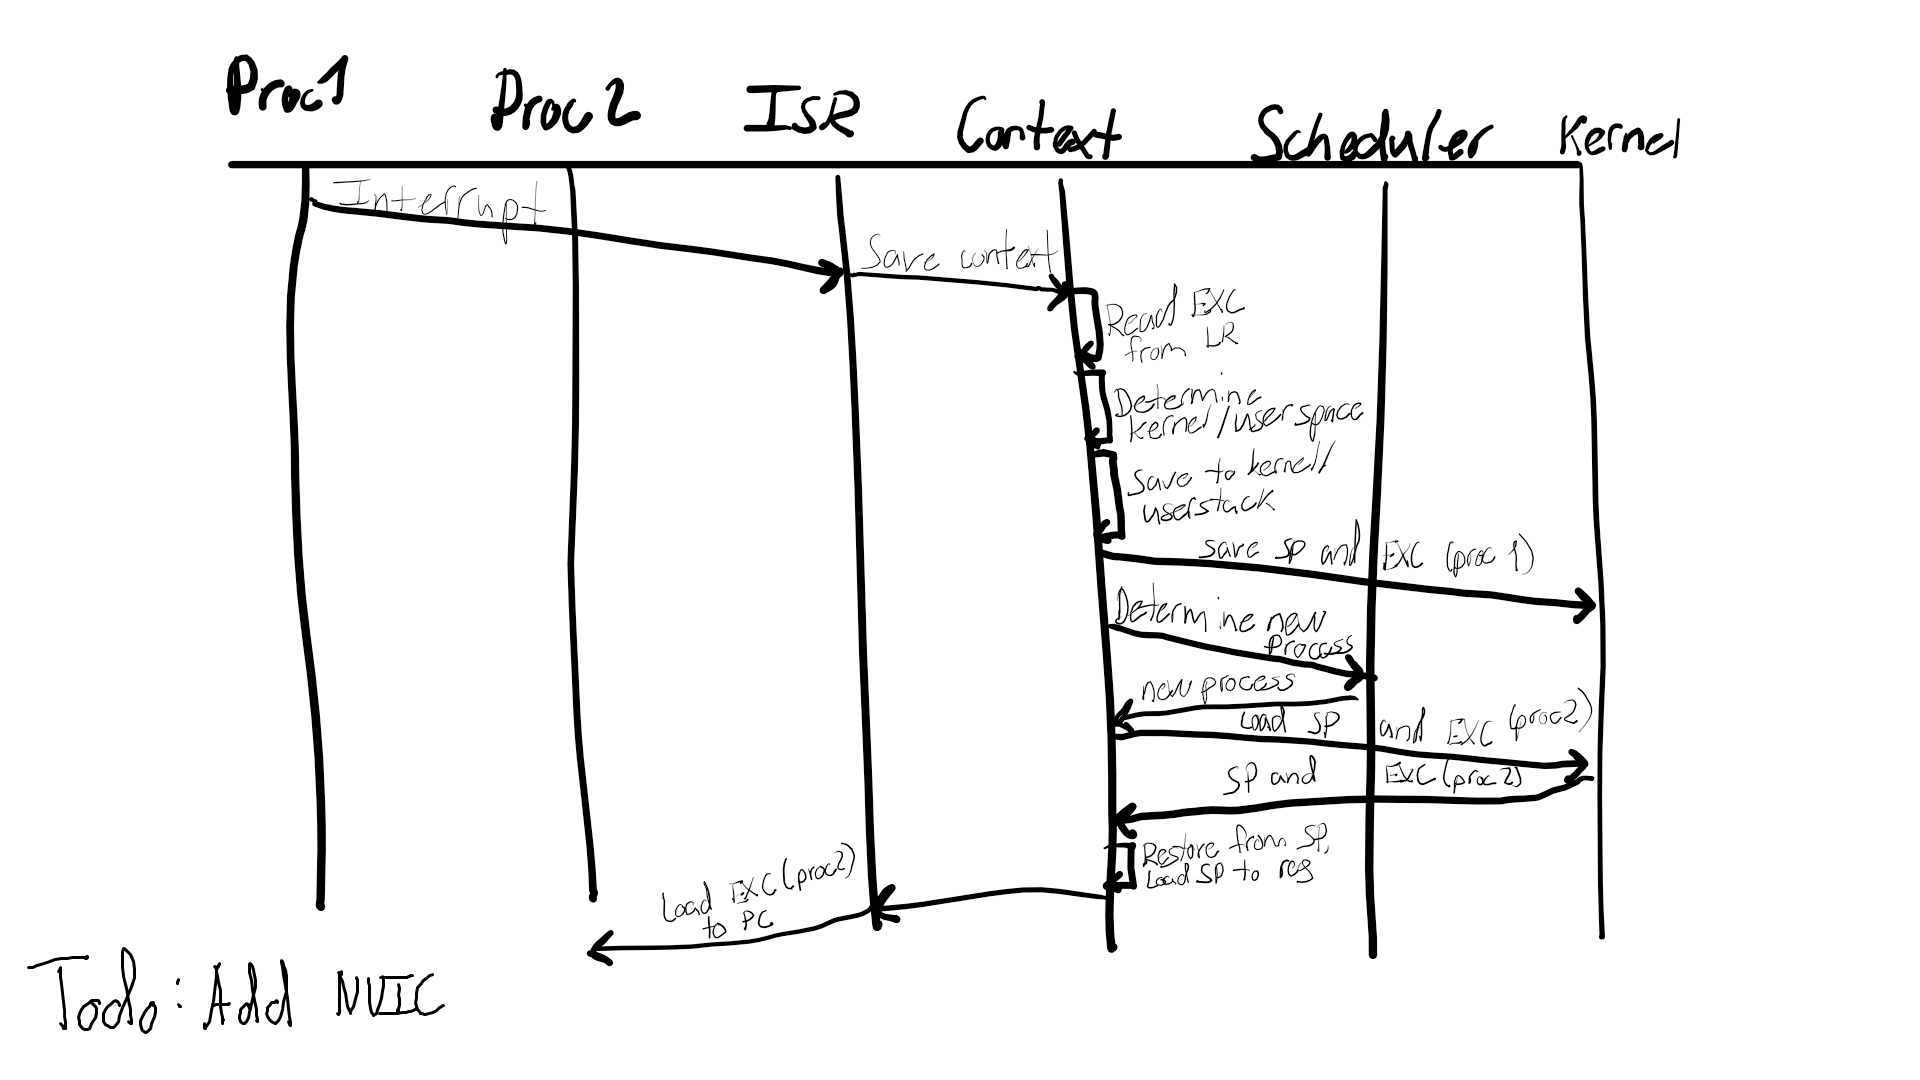
\includegraphics[width=\textwidth]{figures/flowchart_contextswitch.png}
    \caption{This is just a placeholder.}
    \label{fig:flowchart_contextswitch}
\end{figure}

\subsubsection{windows}

\subsubsection{Partition Scheduler}

\subsubsection{Process scheduler}


\subsection{Ports}

\subsubsection{Queuing Ports}
\subsubsection{Sampling Ports}


\subsection{APEX}

\subsubsection{Syscalls}


\subsection{Error Handling}


\section{Partitions and processes}

\subsection{Partitions}

\subsection{Processes}

\subsection{idle\_sys}

\subsection{stdio\_sys}

\subsection{dummy1}

\subsection{dummy2}

\subsection{evil}


\section{Features of the system}
\todo[inline, color=green]{Here we can have a table showing what features
our system has, what features were not implemented, in regards to the
standard}
